\section{Question 2: Results and Comparative Analysis}

\subsection{Performance Across Feature Sets}

Tables~\ref{tab:q2-lr} and \ref{tab:q2-nb} summarize model performance for each feature configuration.

\begin{table}[H]
\centering
\caption{Logistic Regression performance across Q2 feature sets}
\label{tab:q2-lr}
\begin{tabular}{lcccc}
\toprule
Feature set & Acc & Prec & Rec & F1 \\
\midrule
Structural only          & 0.6763 & 0.7042 & 0.6080 & 0.6526 \\
Statistical/content      & 0.6518 & 0.6974 & 0.5363 & 0.6063 \\
Creative handcrafted     & 0.7310 & 0.7750 & 0.6509 & 0.7076 \\
All combined             & 0.7857 & 0.8315 & 0.7165 & 0.7697 \\
\bottomrule
\end{tabular}
\end{table}

\begin{table}[H]
\centering
\caption{Gaussian Naive Bayes performance across Q2 feature sets}
\label{tab:q2-nb}
\begin{tabular}{lcccc}
\toprule
Feature set & Acc & Prec & Rec & F1 \\
\midrule
Structural only          & 0.6824 & 0.8243 & 0.4637 & 0.5935 \\
Statistical/content      & 0.6444 & 0.7696 & 0.4121 & 0.5368 \\
Creative handcrafted     & 0.6601 & 0.9621 & 0.3333 & 0.4951 \\
All combined             & 0.7227 & 0.9442 & 0.4733 & 0.6305 \\
\bottomrule
\end{tabular}
\end{table}

The combined feature configuration is best for both models. Logistic Regression achieves the strongest overall balance, while Naive Bayes tends to exhibit very high precision with noticeably lower recall.

\subsection{Combined-Model Error Decomposition}

Because combined features provide the best headline performance, we inspect their confusion structure directly in Table~\ref{tab:q2-combined-diagnostics}.

\begin{table}[H]
\centering
\caption{Detailed diagnostics on combined features (Q2)}
\label{tab:q2-combined-diagnostics}
\scriptsize
\setlength{\tabcolsep}{3.5pt}
\begin{tabular}{lcc}
\toprule
Metric & Logistic Regression & Gaussian NB \\
\midrule
TN / FP / FN / TP & 977 / 166 / 324 / 819 & 1111 / 32 / 602 / 541 \\
Specificity & 0.8548 & 0.9720 \\
Balanced Accuracy & 0.7857 & 0.7227 \\
MCC & 0.5768 & 0.5138 \\
False Positive Rate & 0.1452 & 0.0280 \\
False Negative Rate & 0.2835 & 0.5267 \\
F1 95\% CI (bootstrap) & [0.7470, 0.7882] & [0.6024, 0.6576] \\
\bottomrule
\end{tabular}
\end{table}

The table clarifies a central tradeoff: Gaussian NB is much more conservative (very low FPR), but it misses a large fraction of true phishing URLs (high FNR). Logistic Regression accepts more false alarms yet recovers substantially more positives, yielding better balanced accuracy and F1.

\subsection{Relative Gain Analysis Across Feature Families}

To quantify feature-engineering value, we compare the best and weakest feature families:
\begin{itemize}
    \item Logistic Regression F1 improves from 0.6063 (statistical/content) to 0.7697 (combined), a +26.96\% relative gain.
    \item Logistic Regression recall improves from 0.5363 to 0.7165, a +33.61\% relative gain.
    \item Naive Bayes F1 improves from 0.5368 (statistical/content) to 0.6305 (combined), a +17.46\% relative gain.
    \item Naive Bayes recall improves from 0.4121 to 0.4733, a +14.85\% relative gain.
\end{itemize}

These improvements indicate that engineering richer feature views has larger impact than changing linear-probabilistic baseline type alone.

\subsection{Distributional and Correlation Insights}

\begin{figure}[H]
\centering
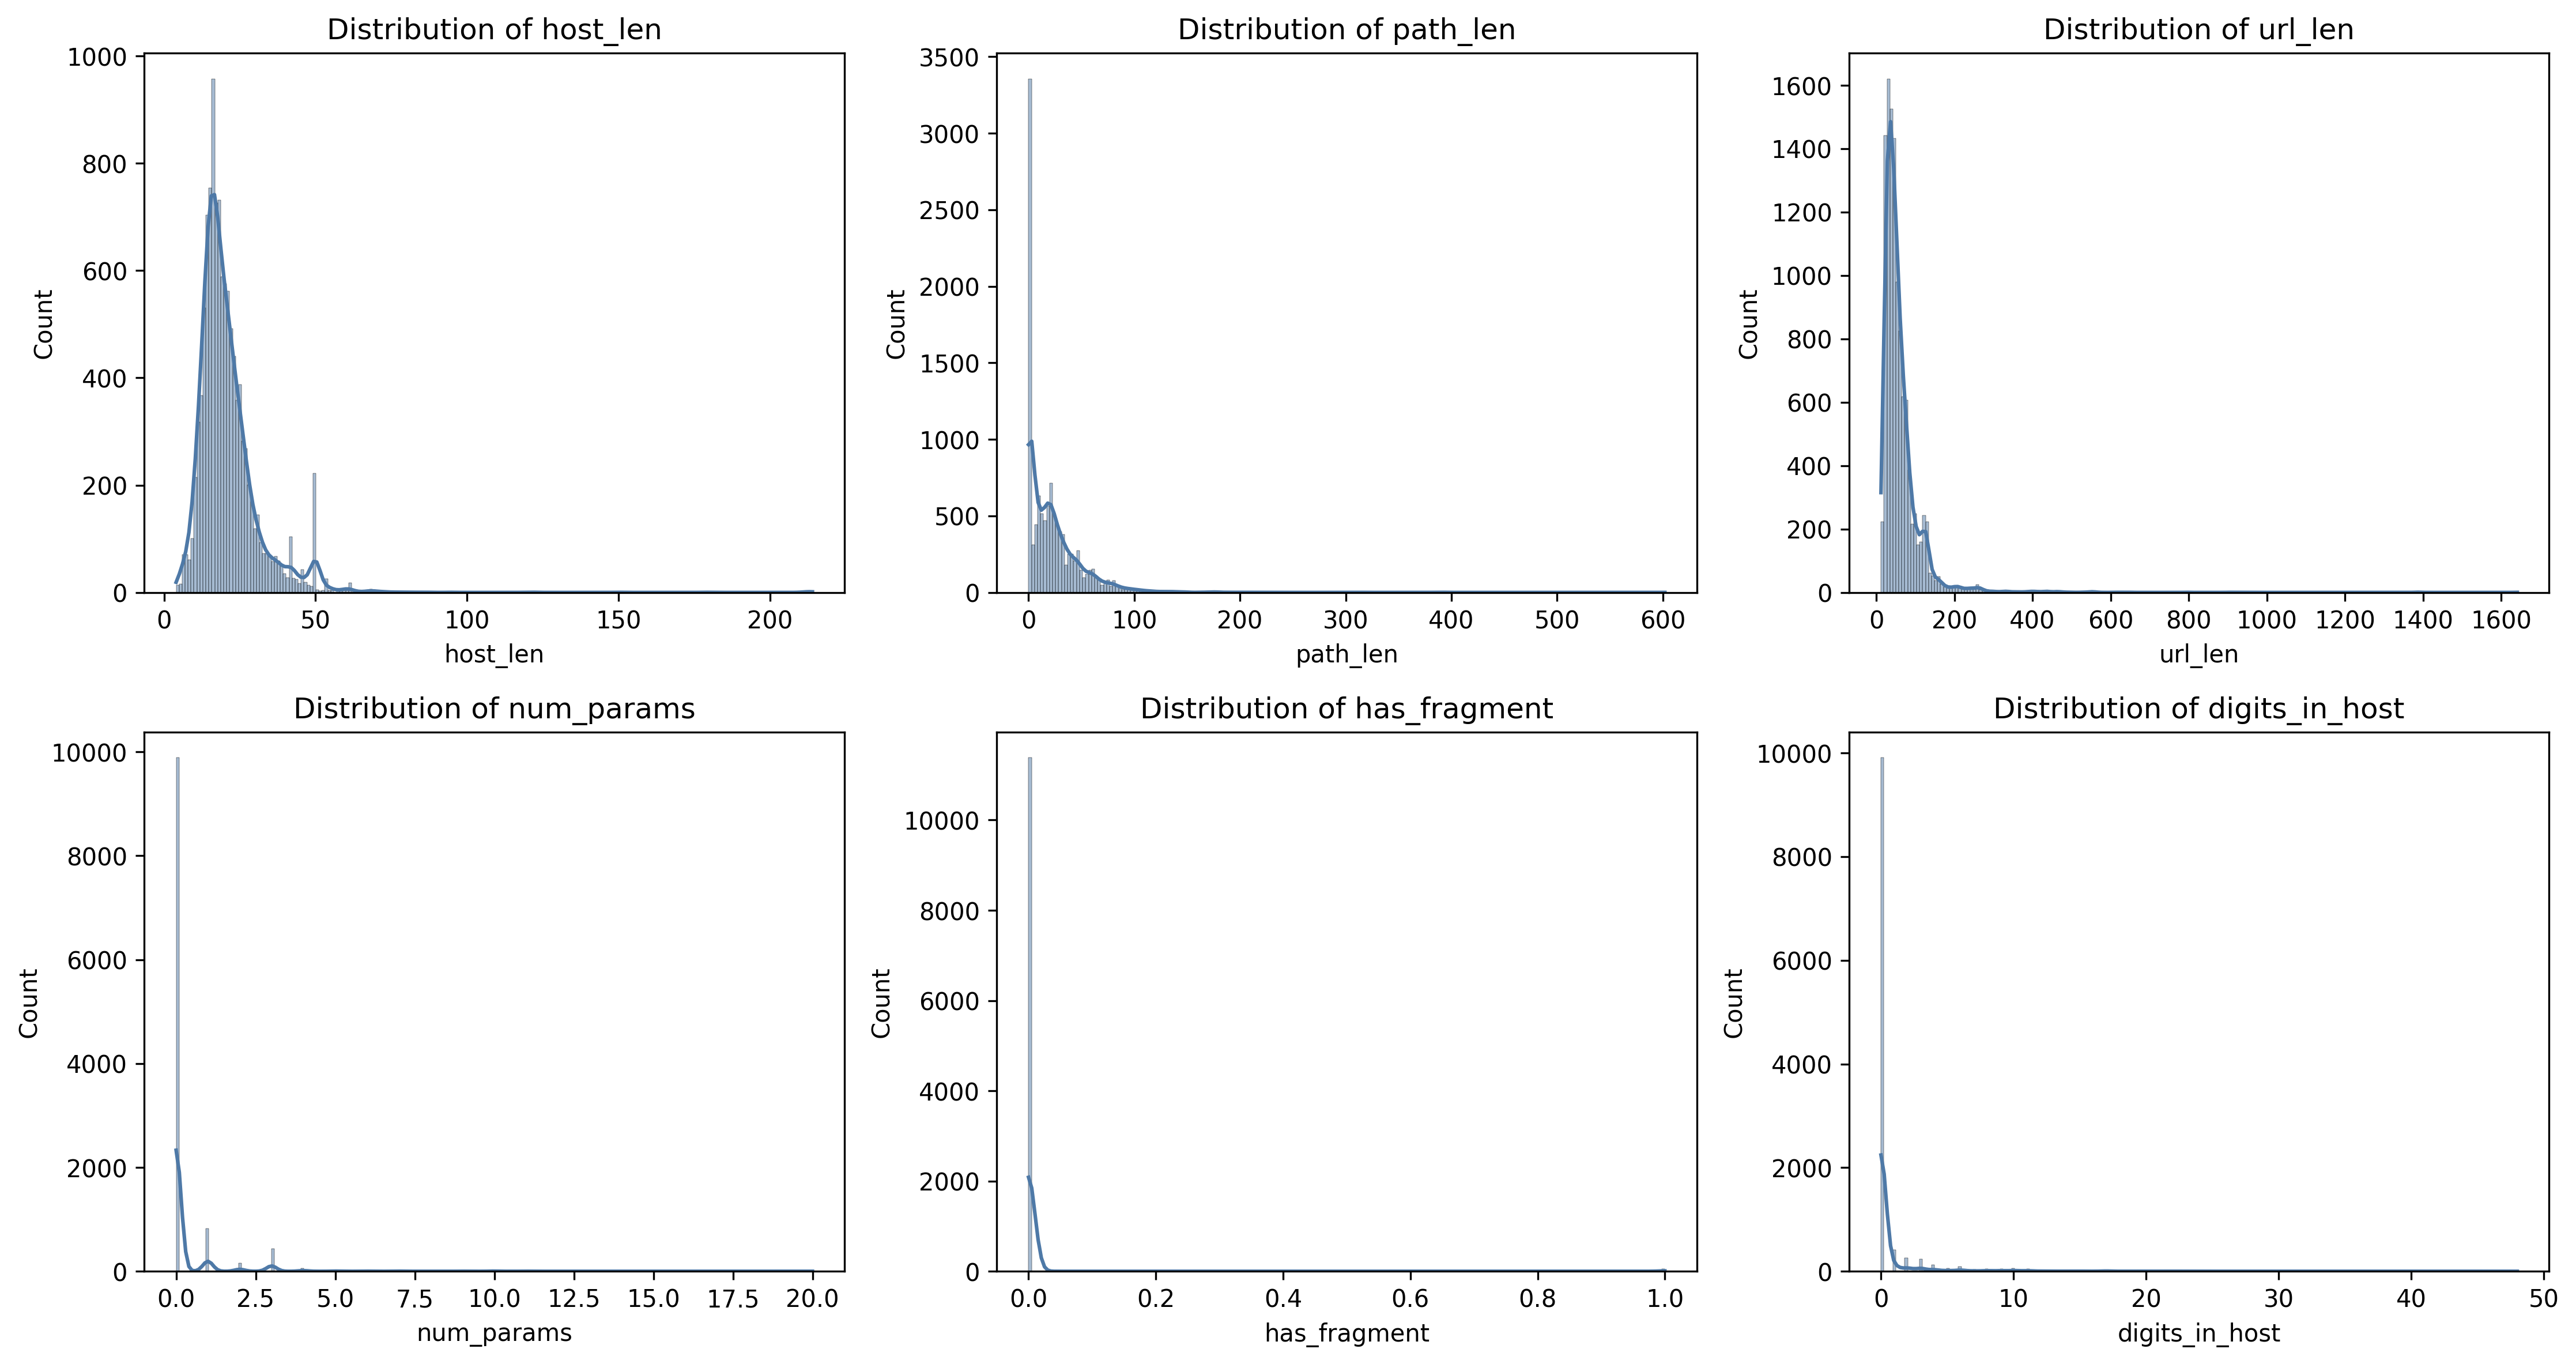
\includegraphics[width=0.48\textwidth]{figures/q2_structural_distributions.png}
\caption{Distributions of structural URL attributes.}
\label{fig:q2-struct-dist}
\end{figure}

\begin{figure}[H]
\centering
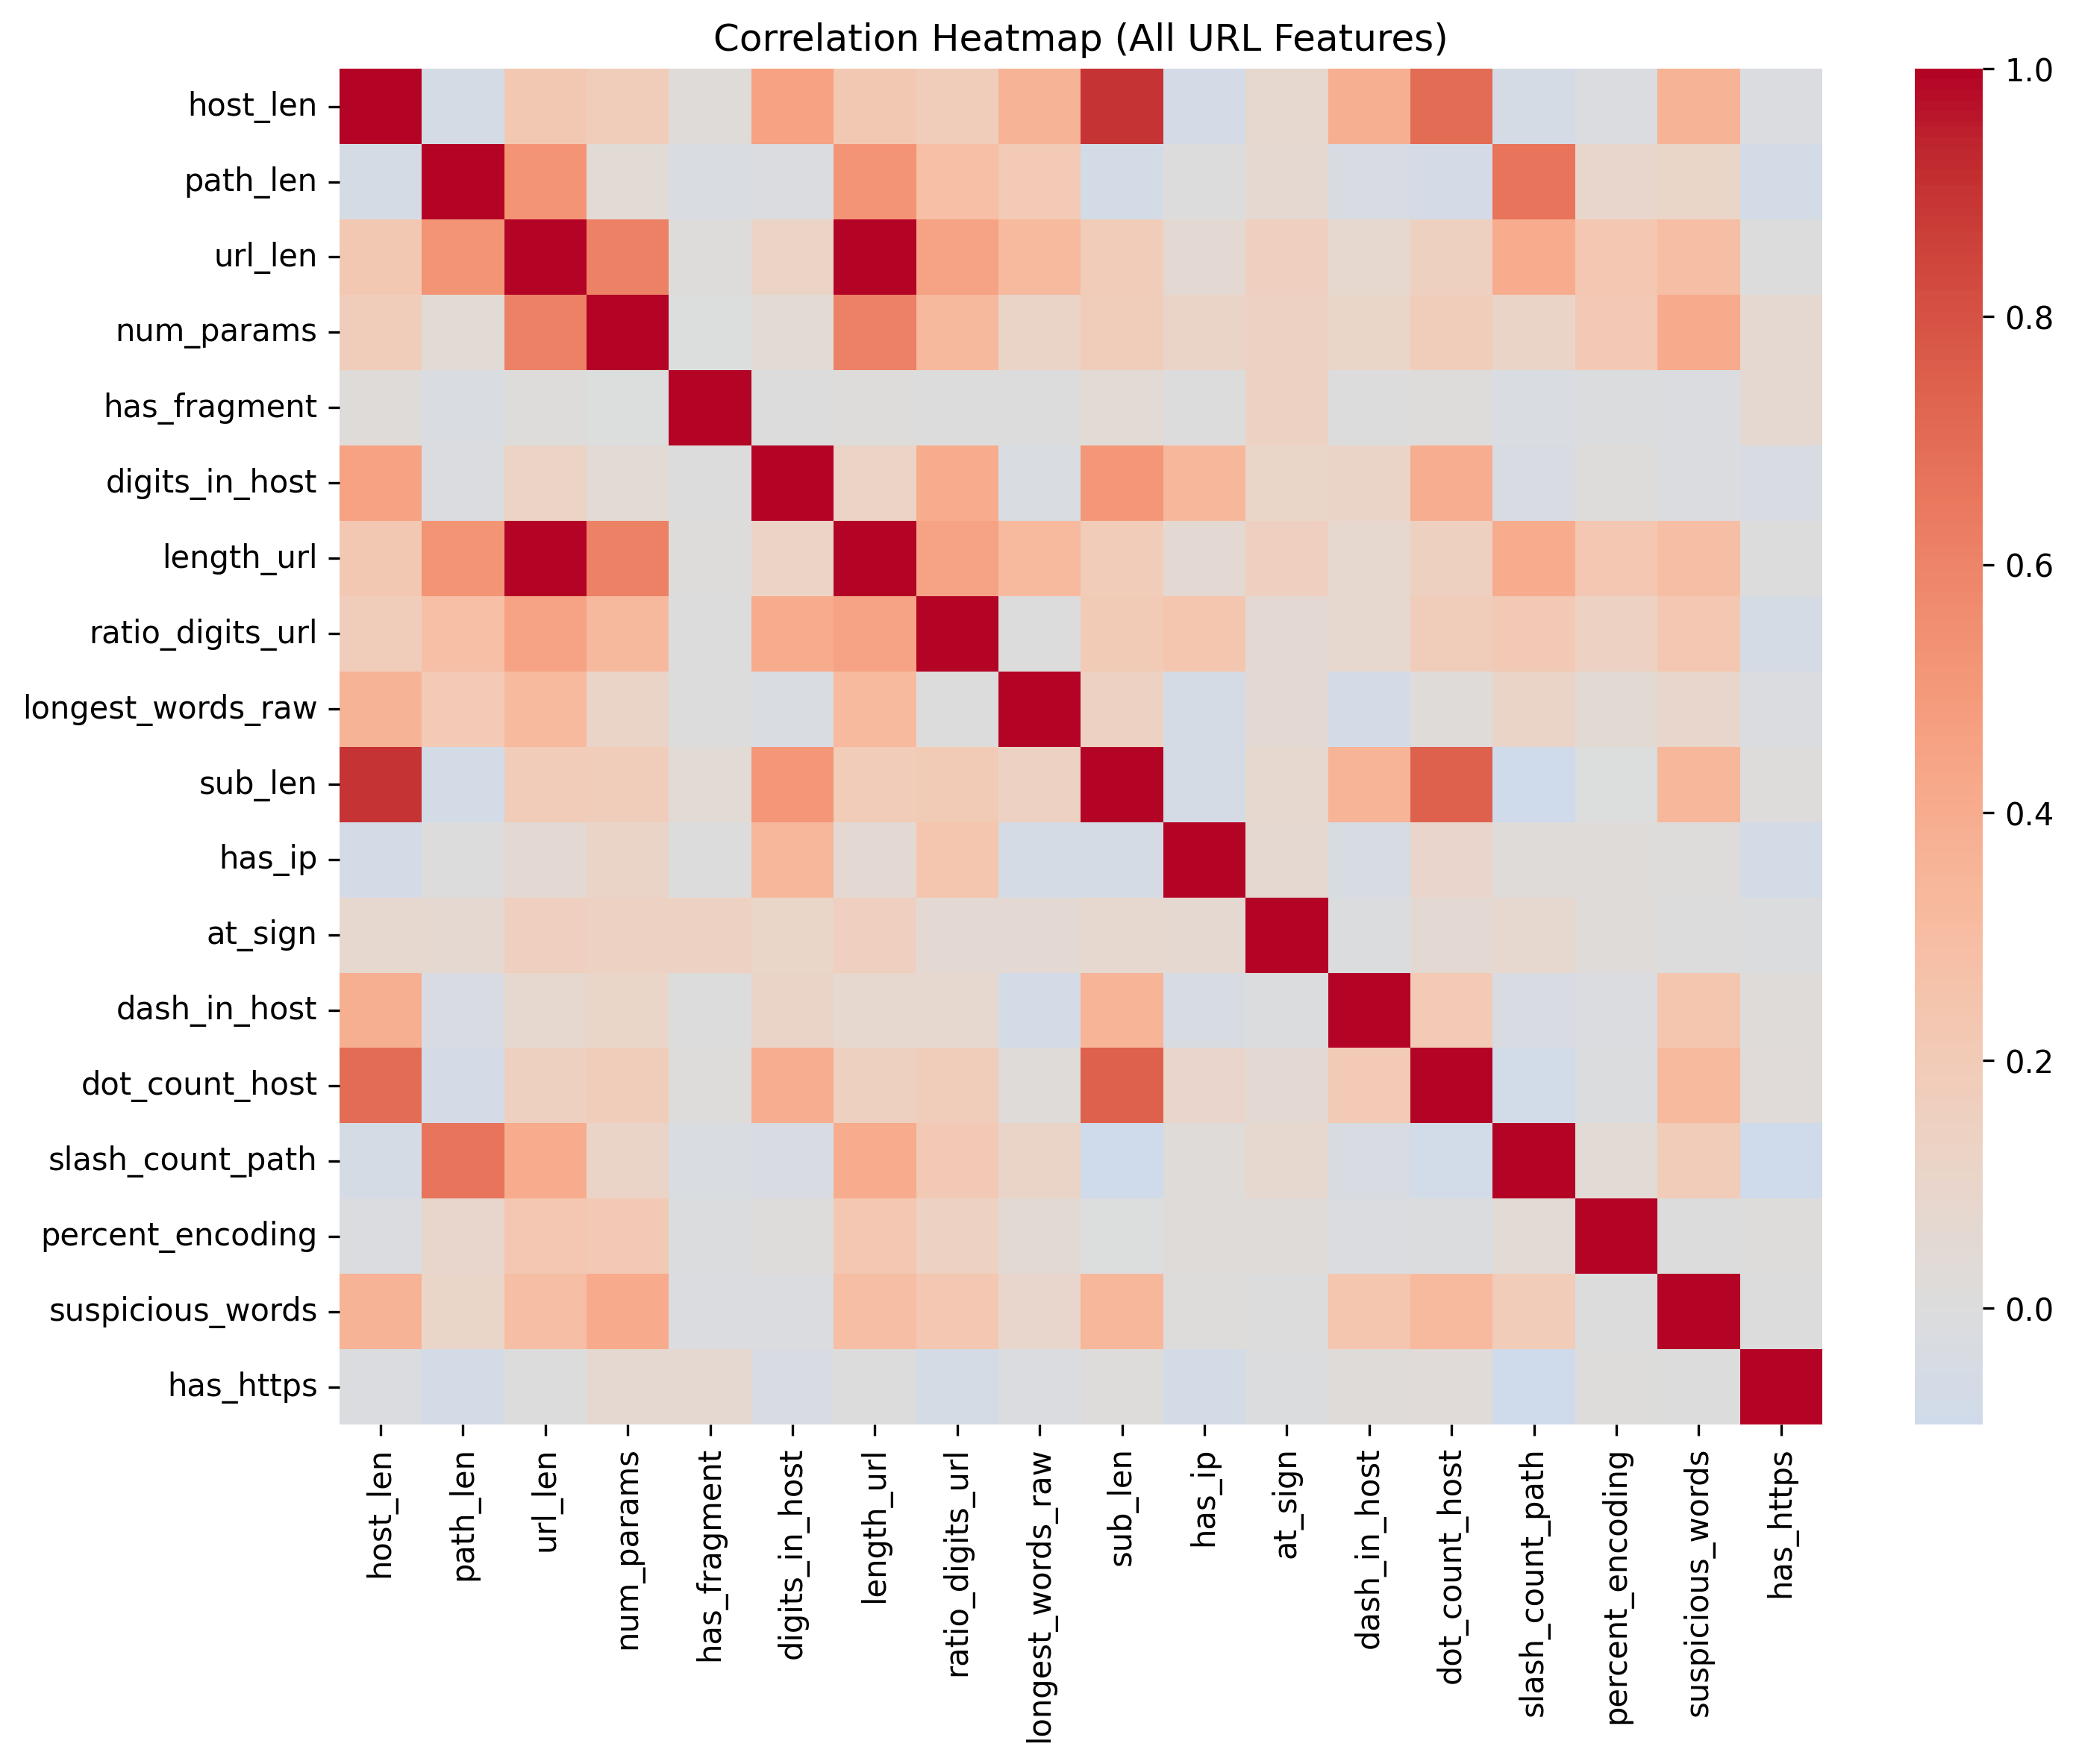
\includegraphics[width=0.48\textwidth]{figures/q2_correlation_heatmap_all_features.png}
\caption{Correlation heatmap of combined URL features.}
\label{fig:q2-corr}
\end{figure}

Figures~\ref{fig:q2-struct-dist} and \ref{fig:q2-corr} reveal moderate inter-feature dependency, indicating that combining views (length, host composition, token patterns) is likely to improve discriminative learning.

\begin{figure}[H]
\centering
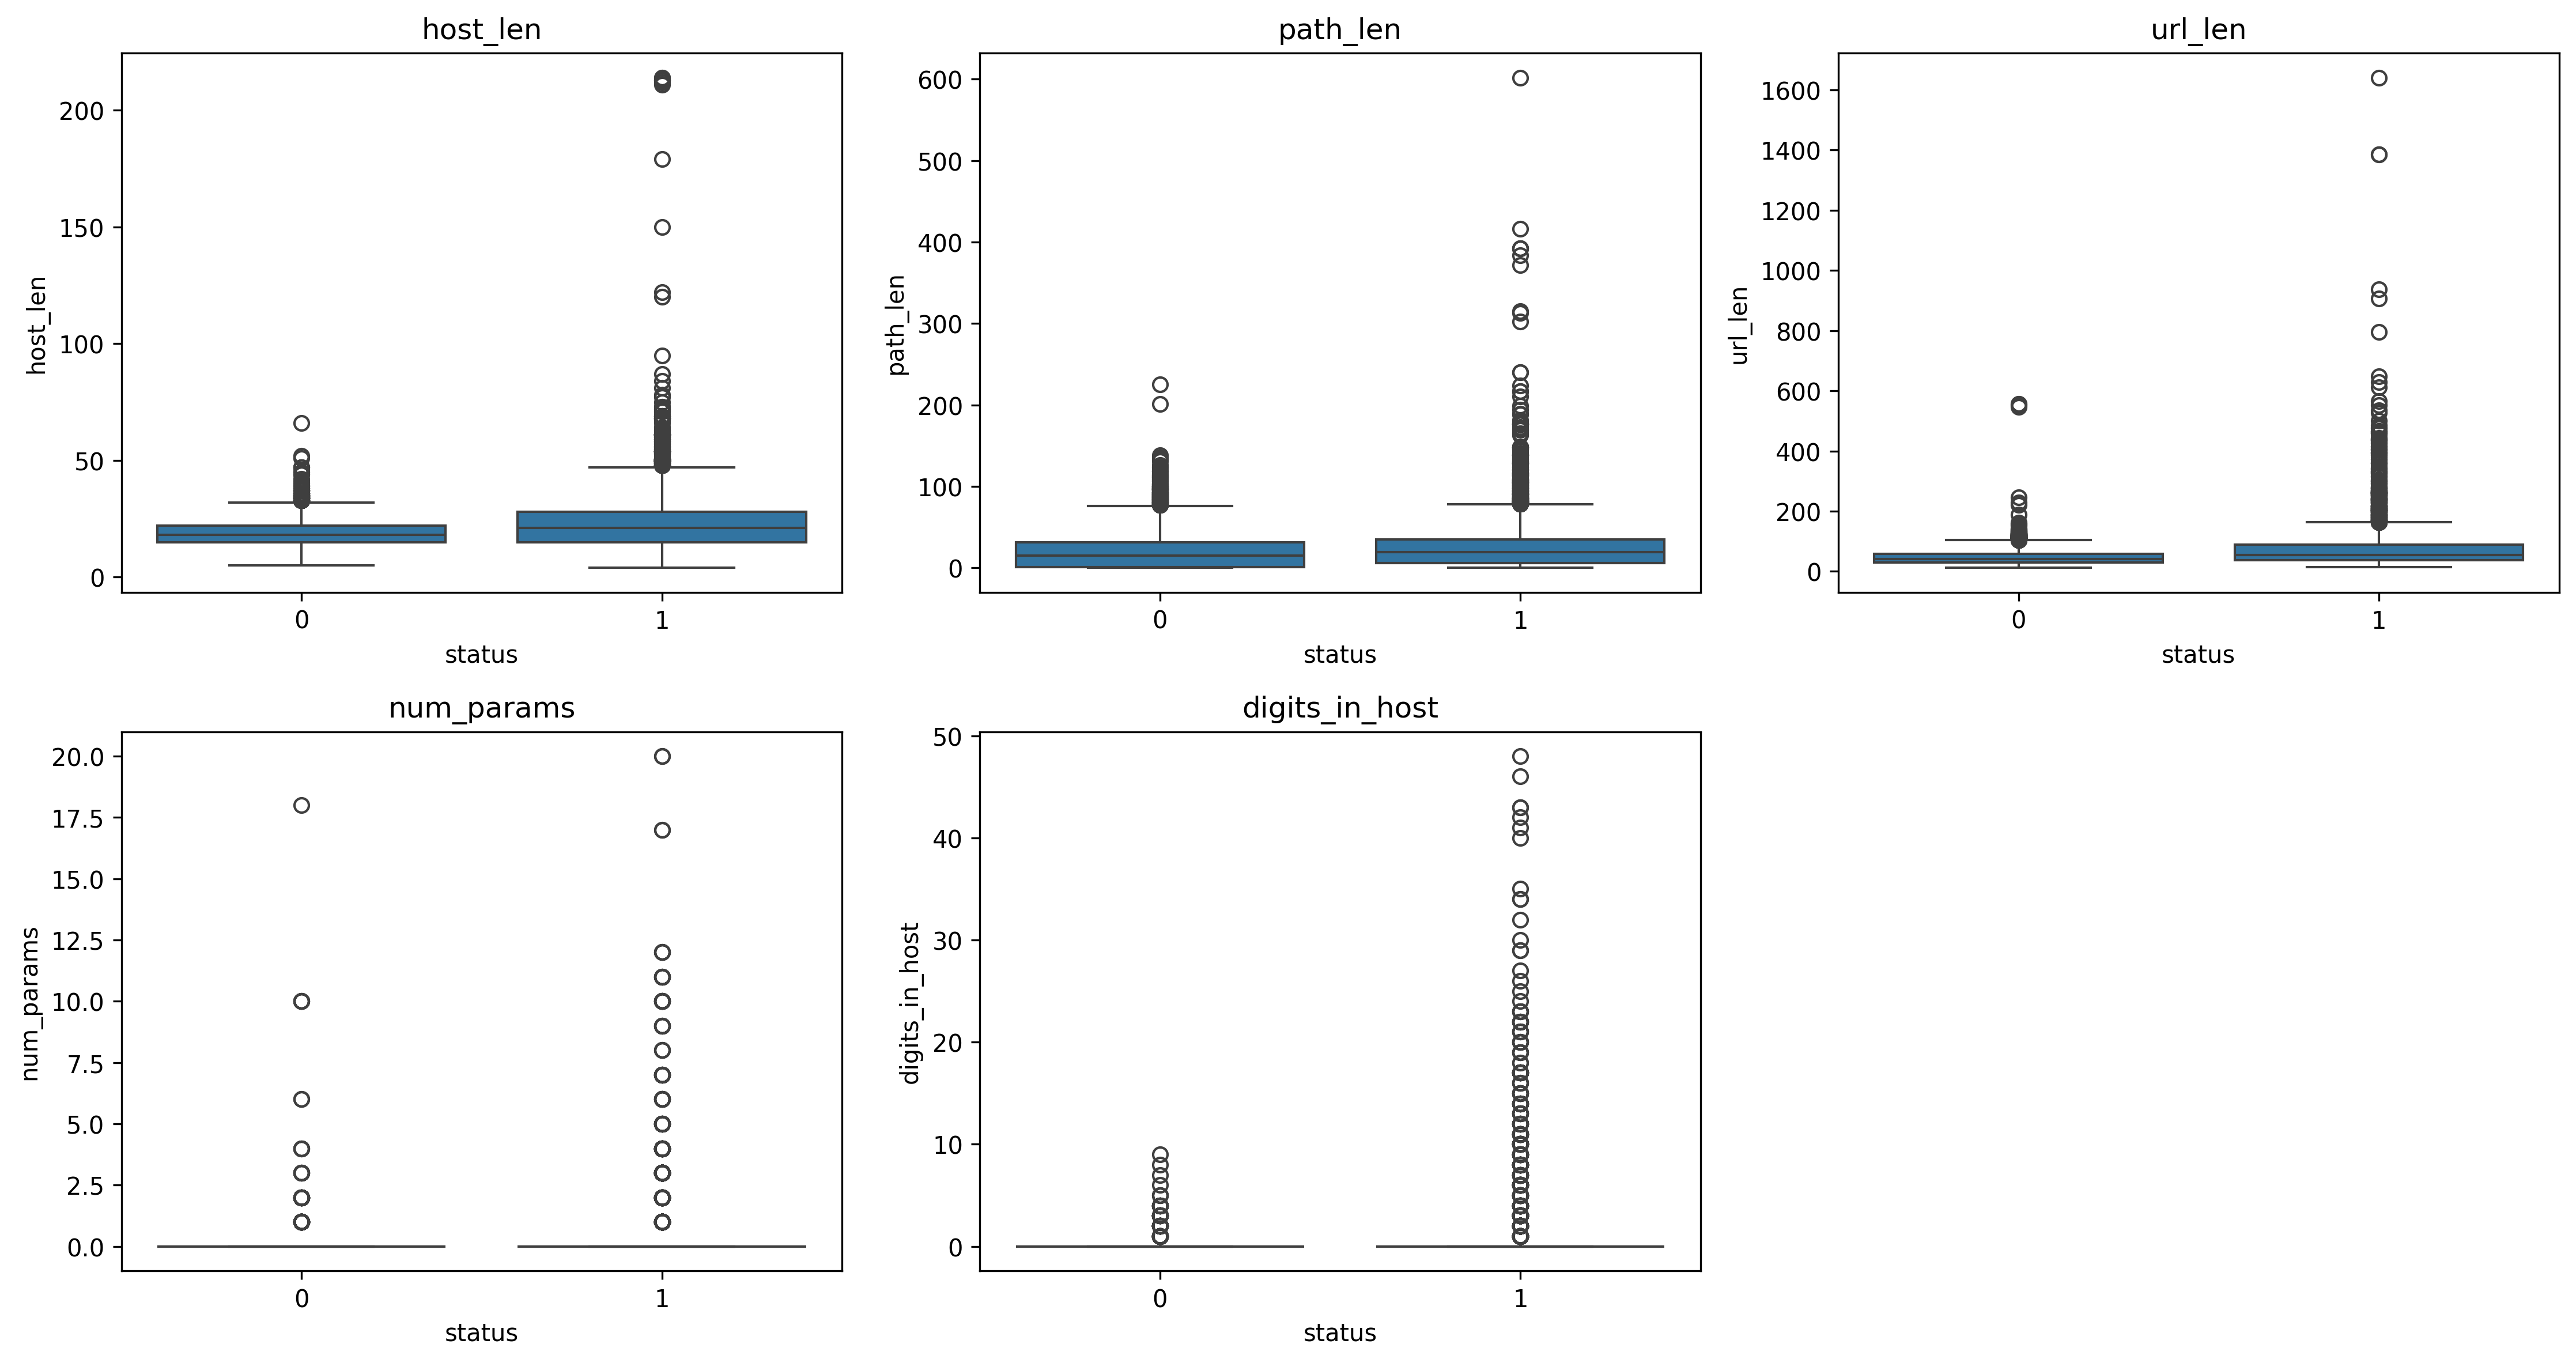
\includegraphics[width=0.48\textwidth]{figures/q2_structural_boxplots.png}
\caption{Structural feature separation by class label.}
\label{fig:q2-box}
\end{figure}

\begin{figure}[H]
\centering
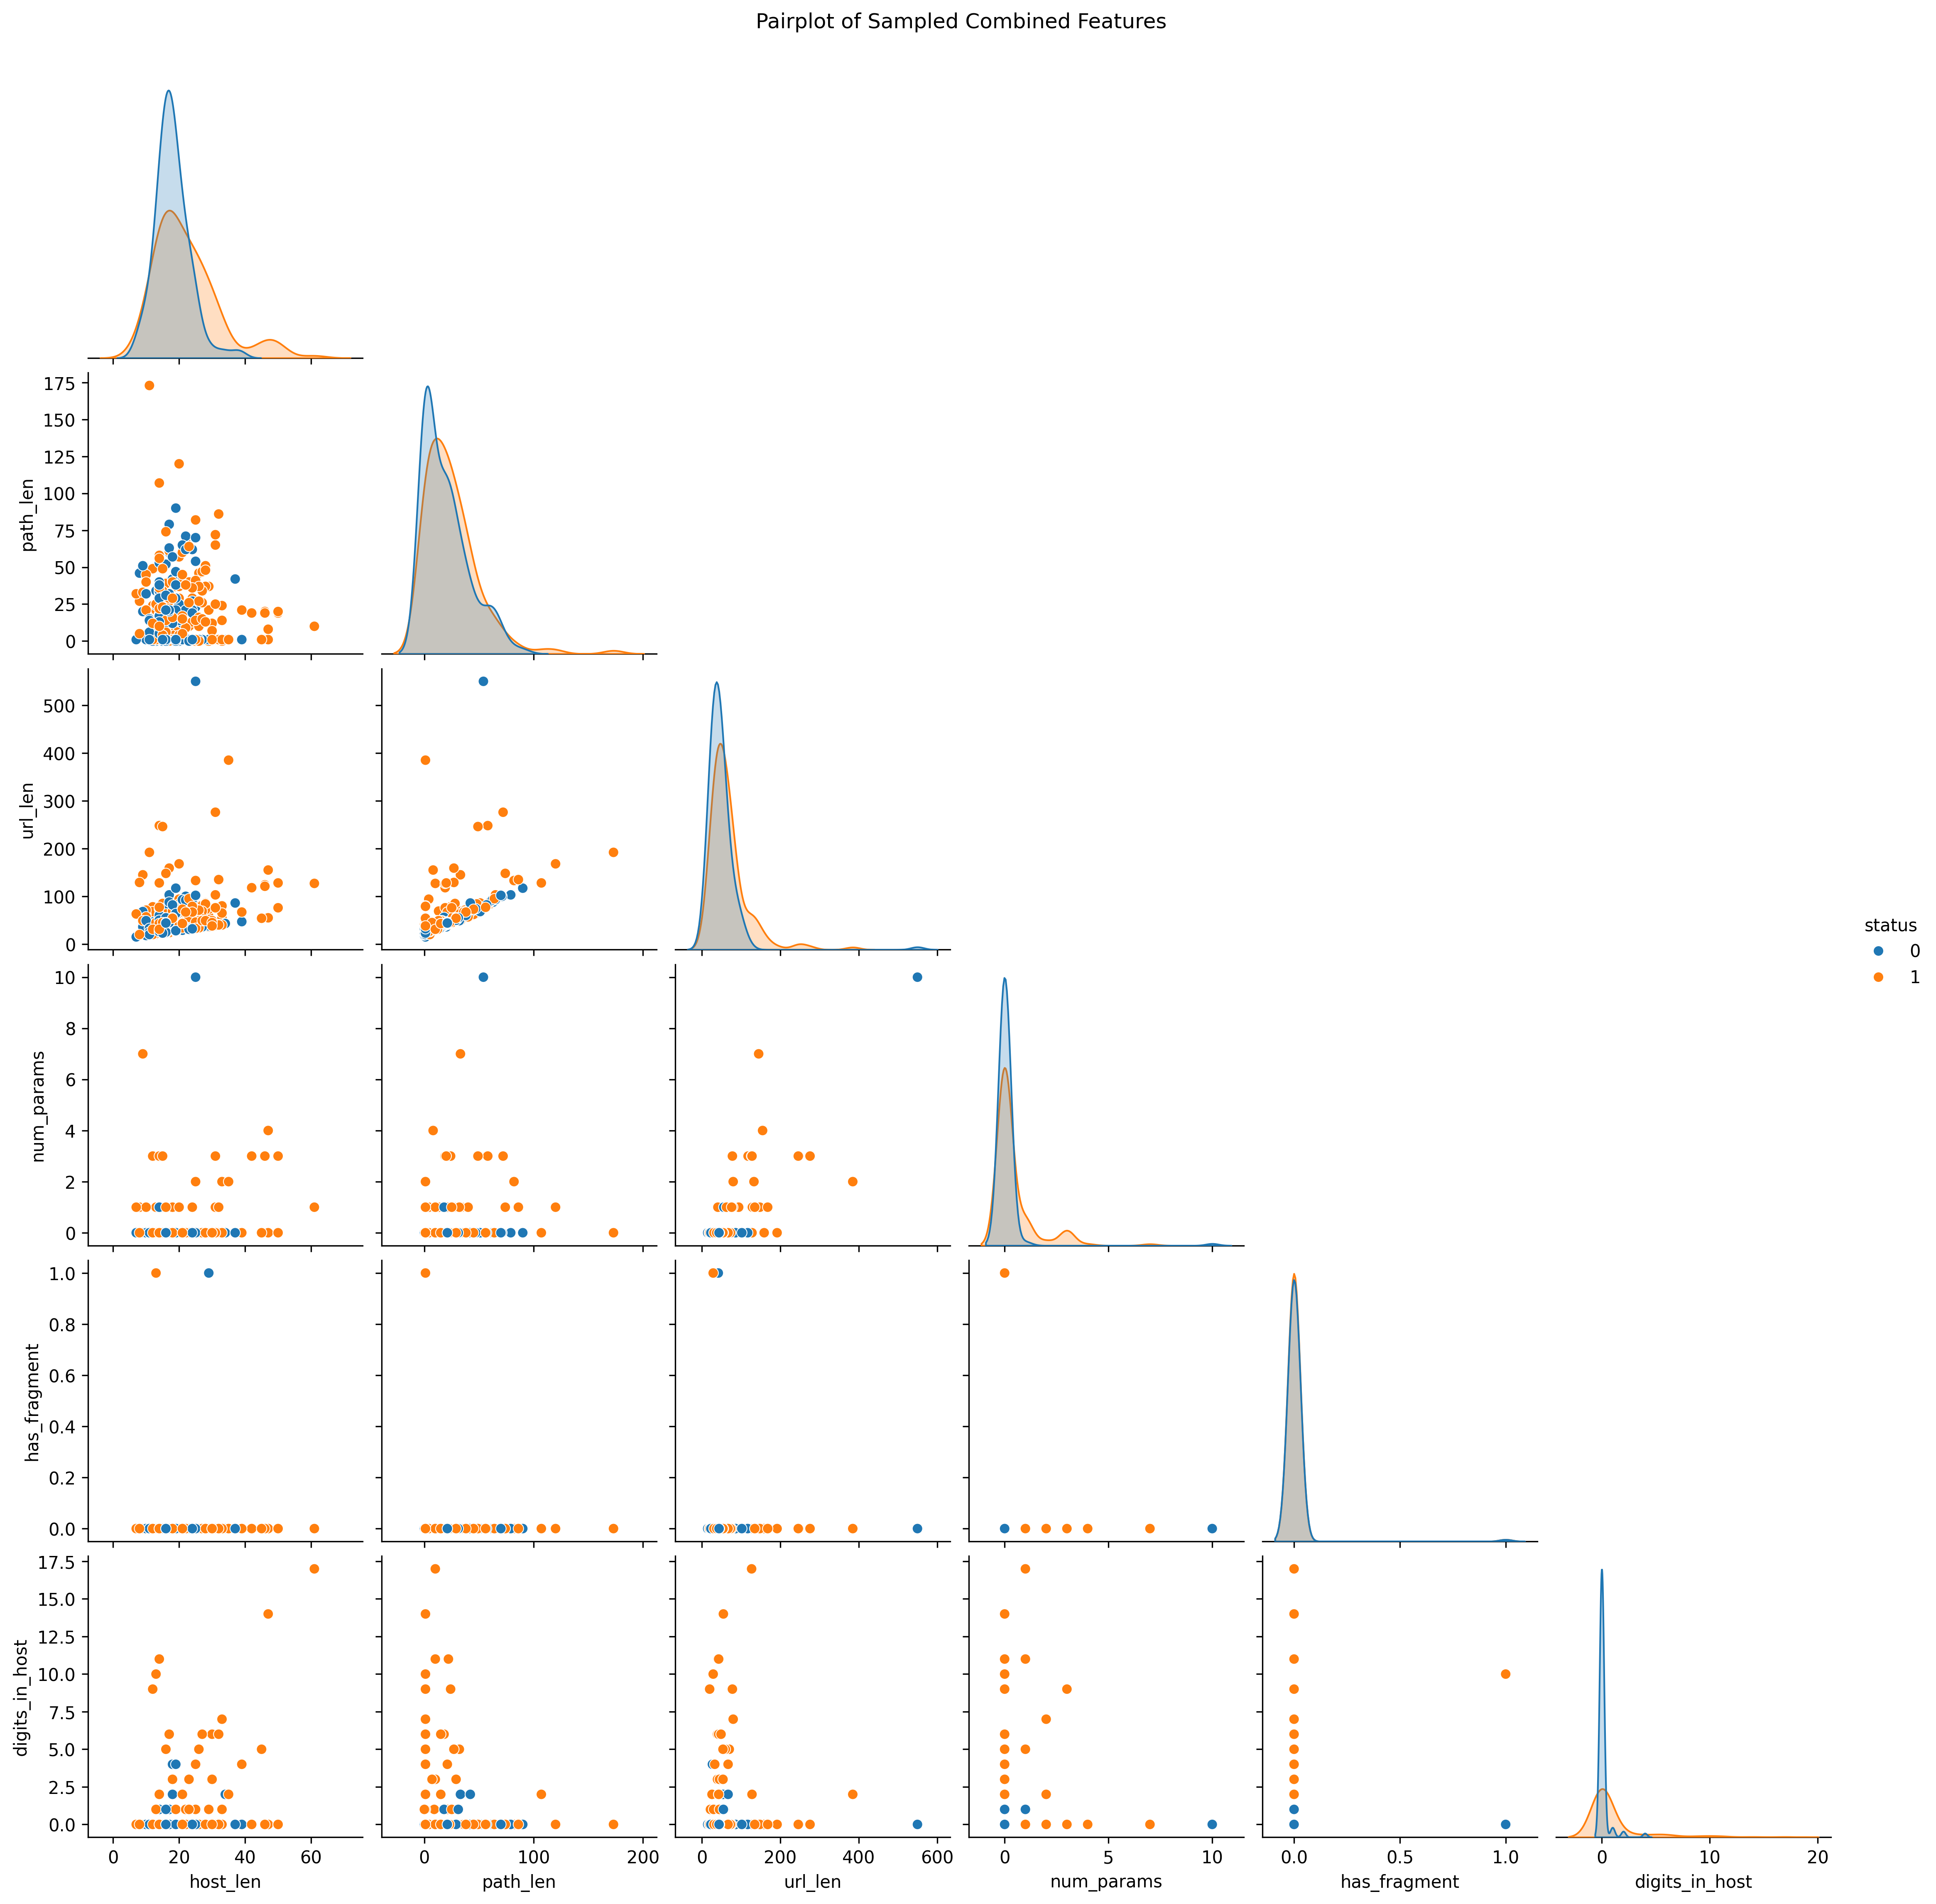
\includegraphics[width=0.48\textwidth]{figures/q2_pairplot_sample.png}
\caption{Pairwise view of sampled combined features.}
\label{fig:q2-pair}
\end{figure}

The boxplot and pairplot views in Figures~\ref{fig:q2-box} and \ref{fig:q2-pair} show partial class overlap but meaningful margin shifts in several dimensions, supporting the improvements observed in the combined setup.

\subsection{Feature Importance and Ranking Curves}

\begin{figure}[H]
\centering
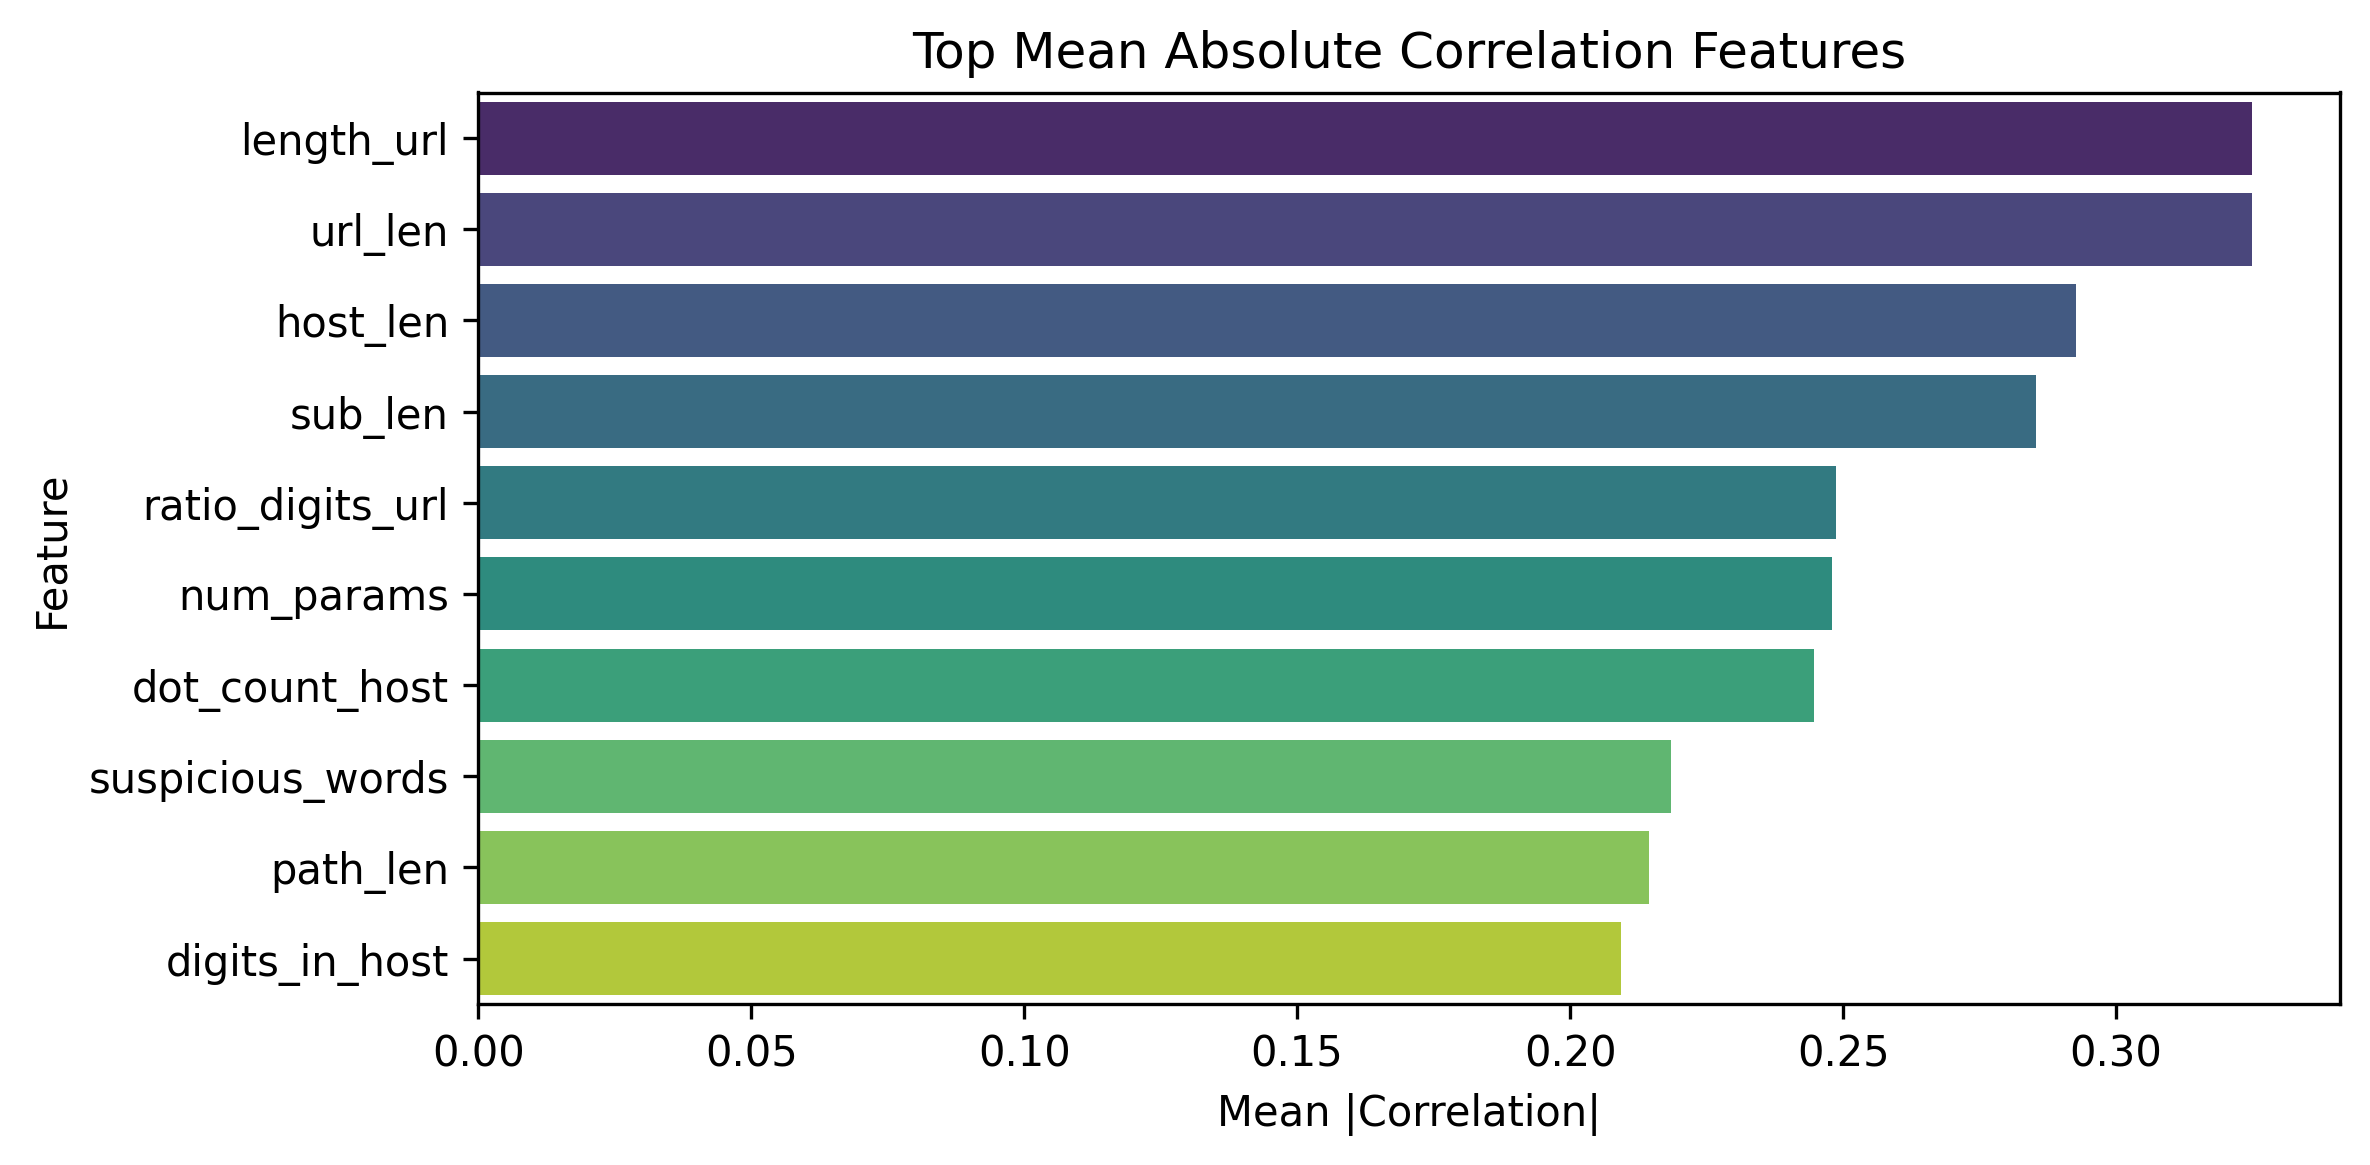
\includegraphics[width=0.48\textwidth]{figures/q2_top_mean_abs_correlations.png}
\caption{Top features by mean absolute correlation.}
\label{fig:q2-topcorr}
\end{figure}

\begin{figure}[H]
\centering
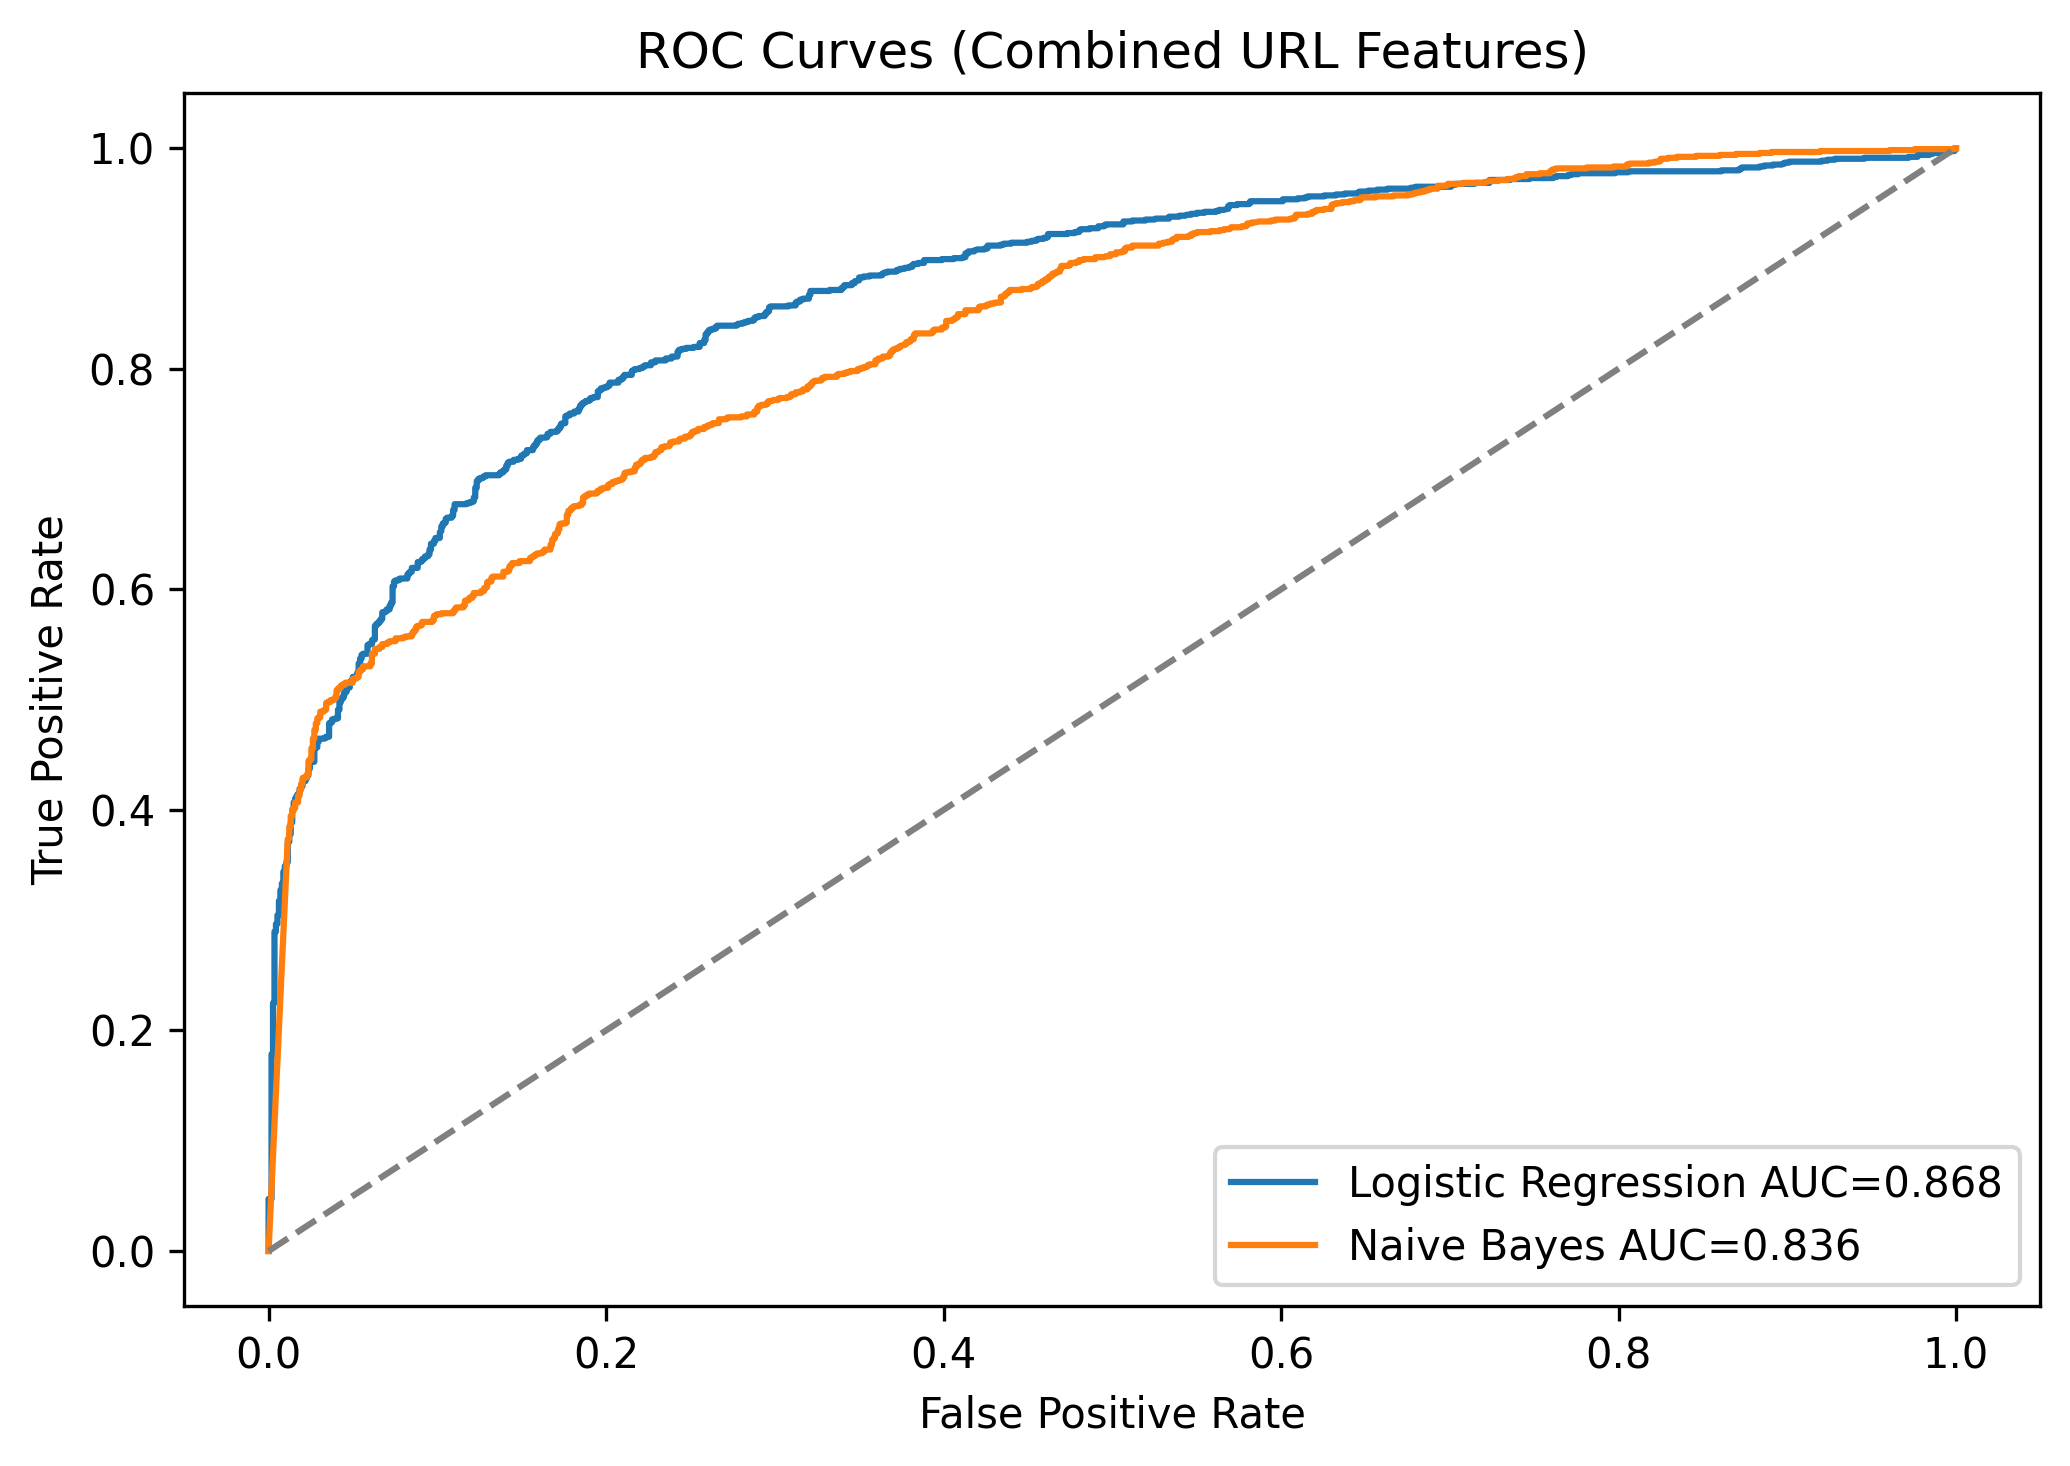
\includegraphics[width=0.48\textwidth]{figures/q2_roc_combined_features.png}
\caption{ROC comparison on combined features.}
\label{fig:q2-roc}
\end{figure}

\begin{figure}[H]
\centering
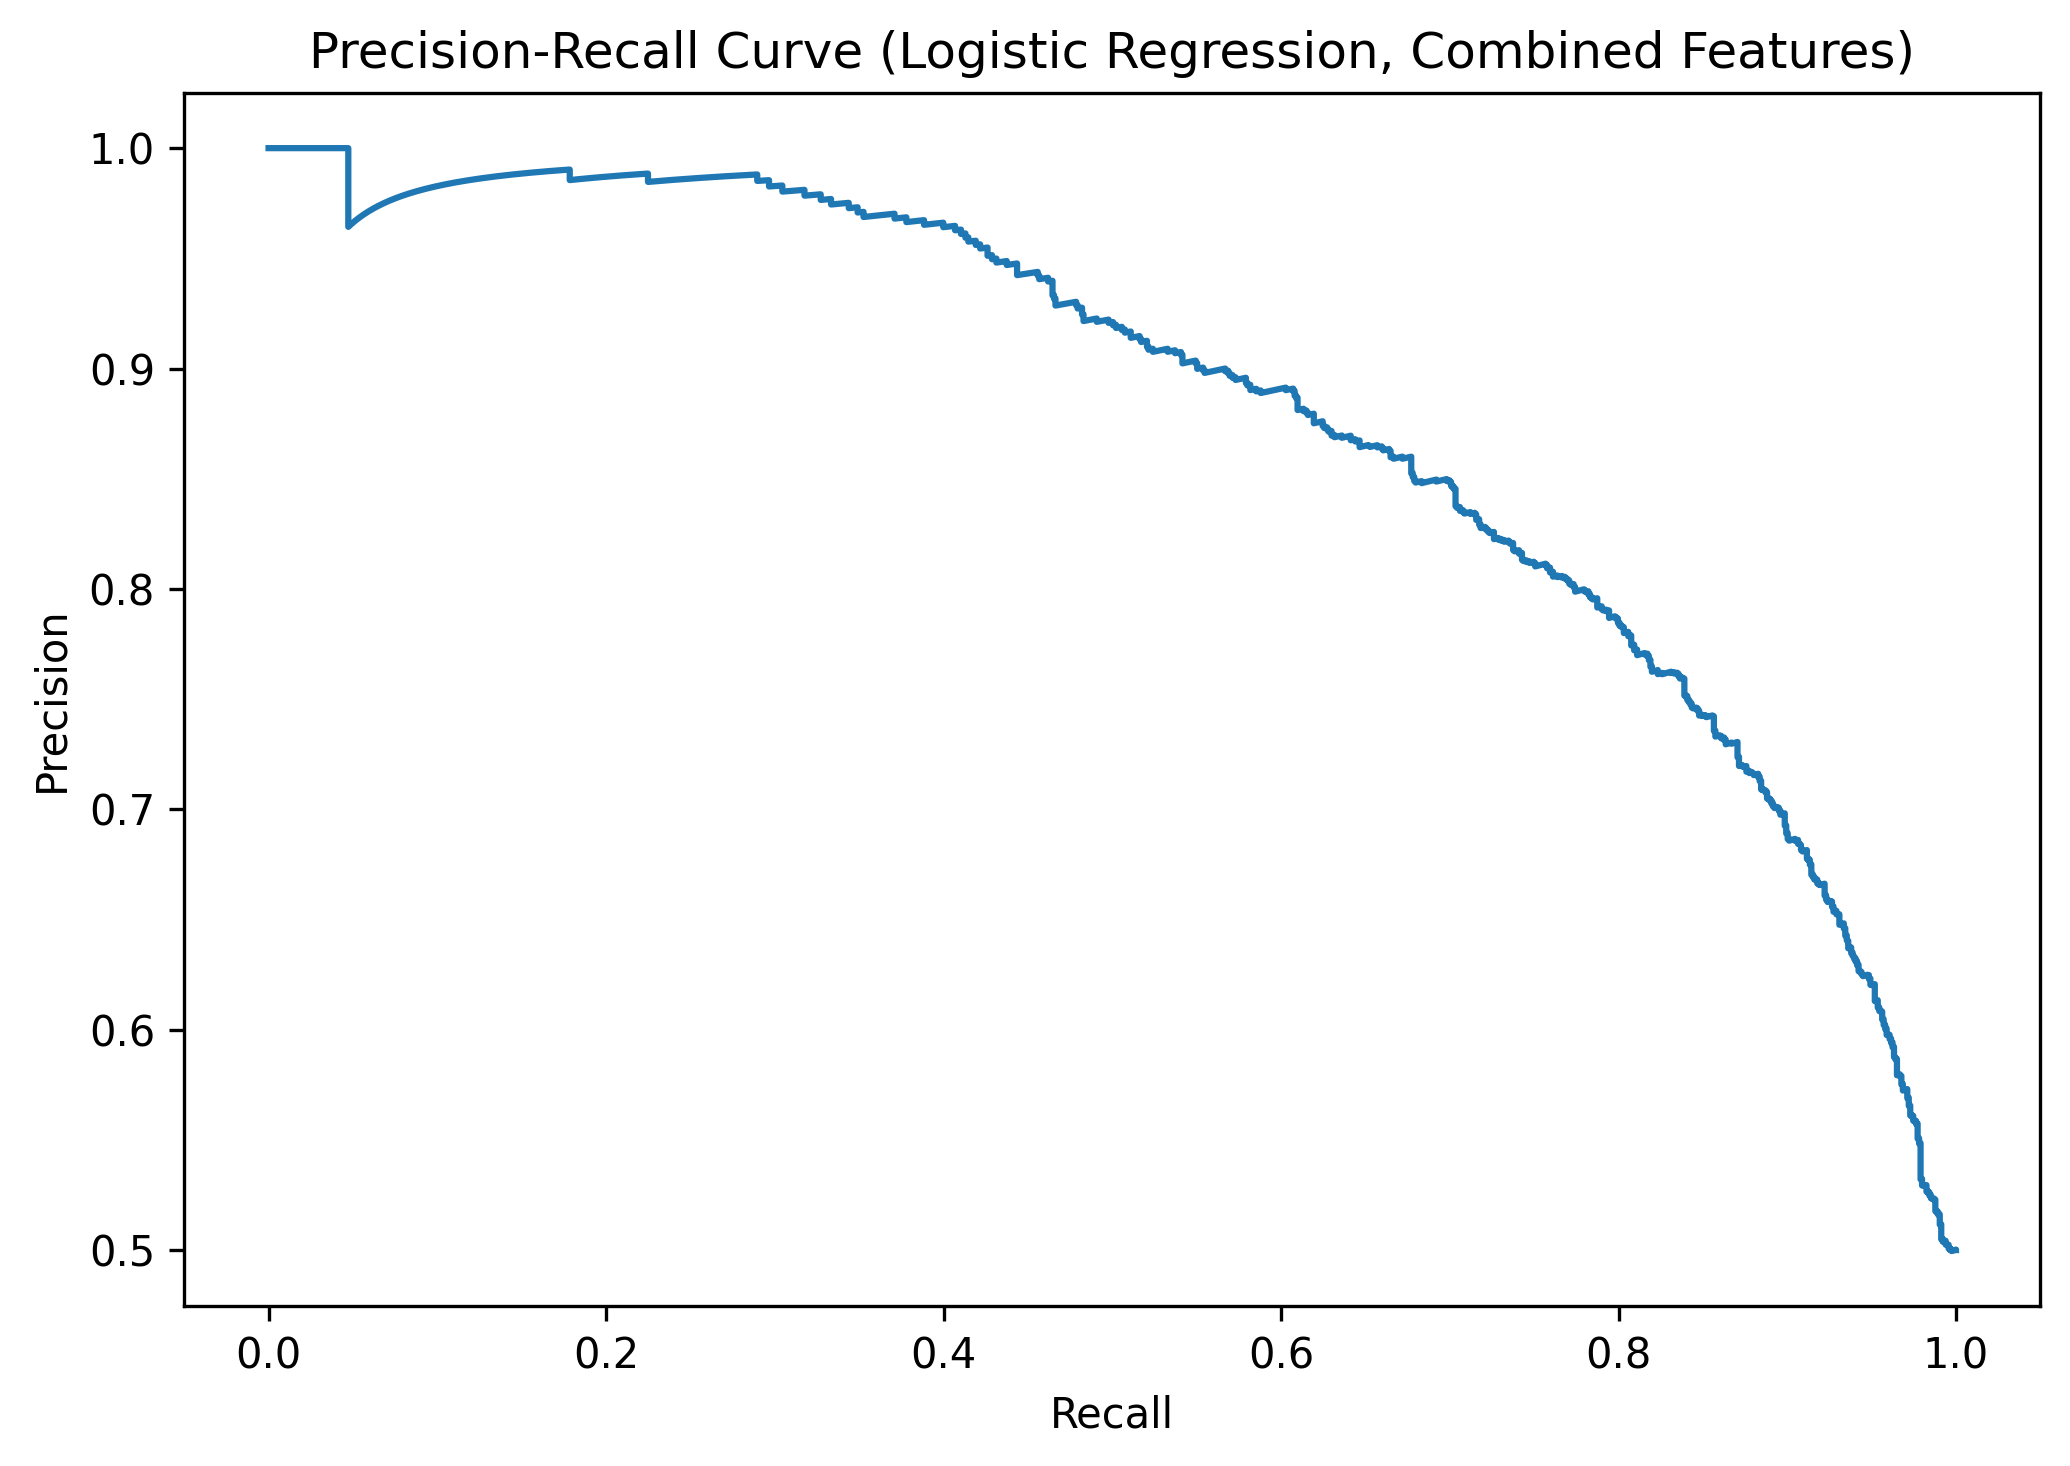
\includegraphics[width=0.48\textwidth]{figures/q2_pr_combined_lr.png}
\caption{Precision-Recall curve for Logistic Regression (combined).}
\label{fig:q2-pr}
\end{figure}

\begin{figure}[H]
\centering
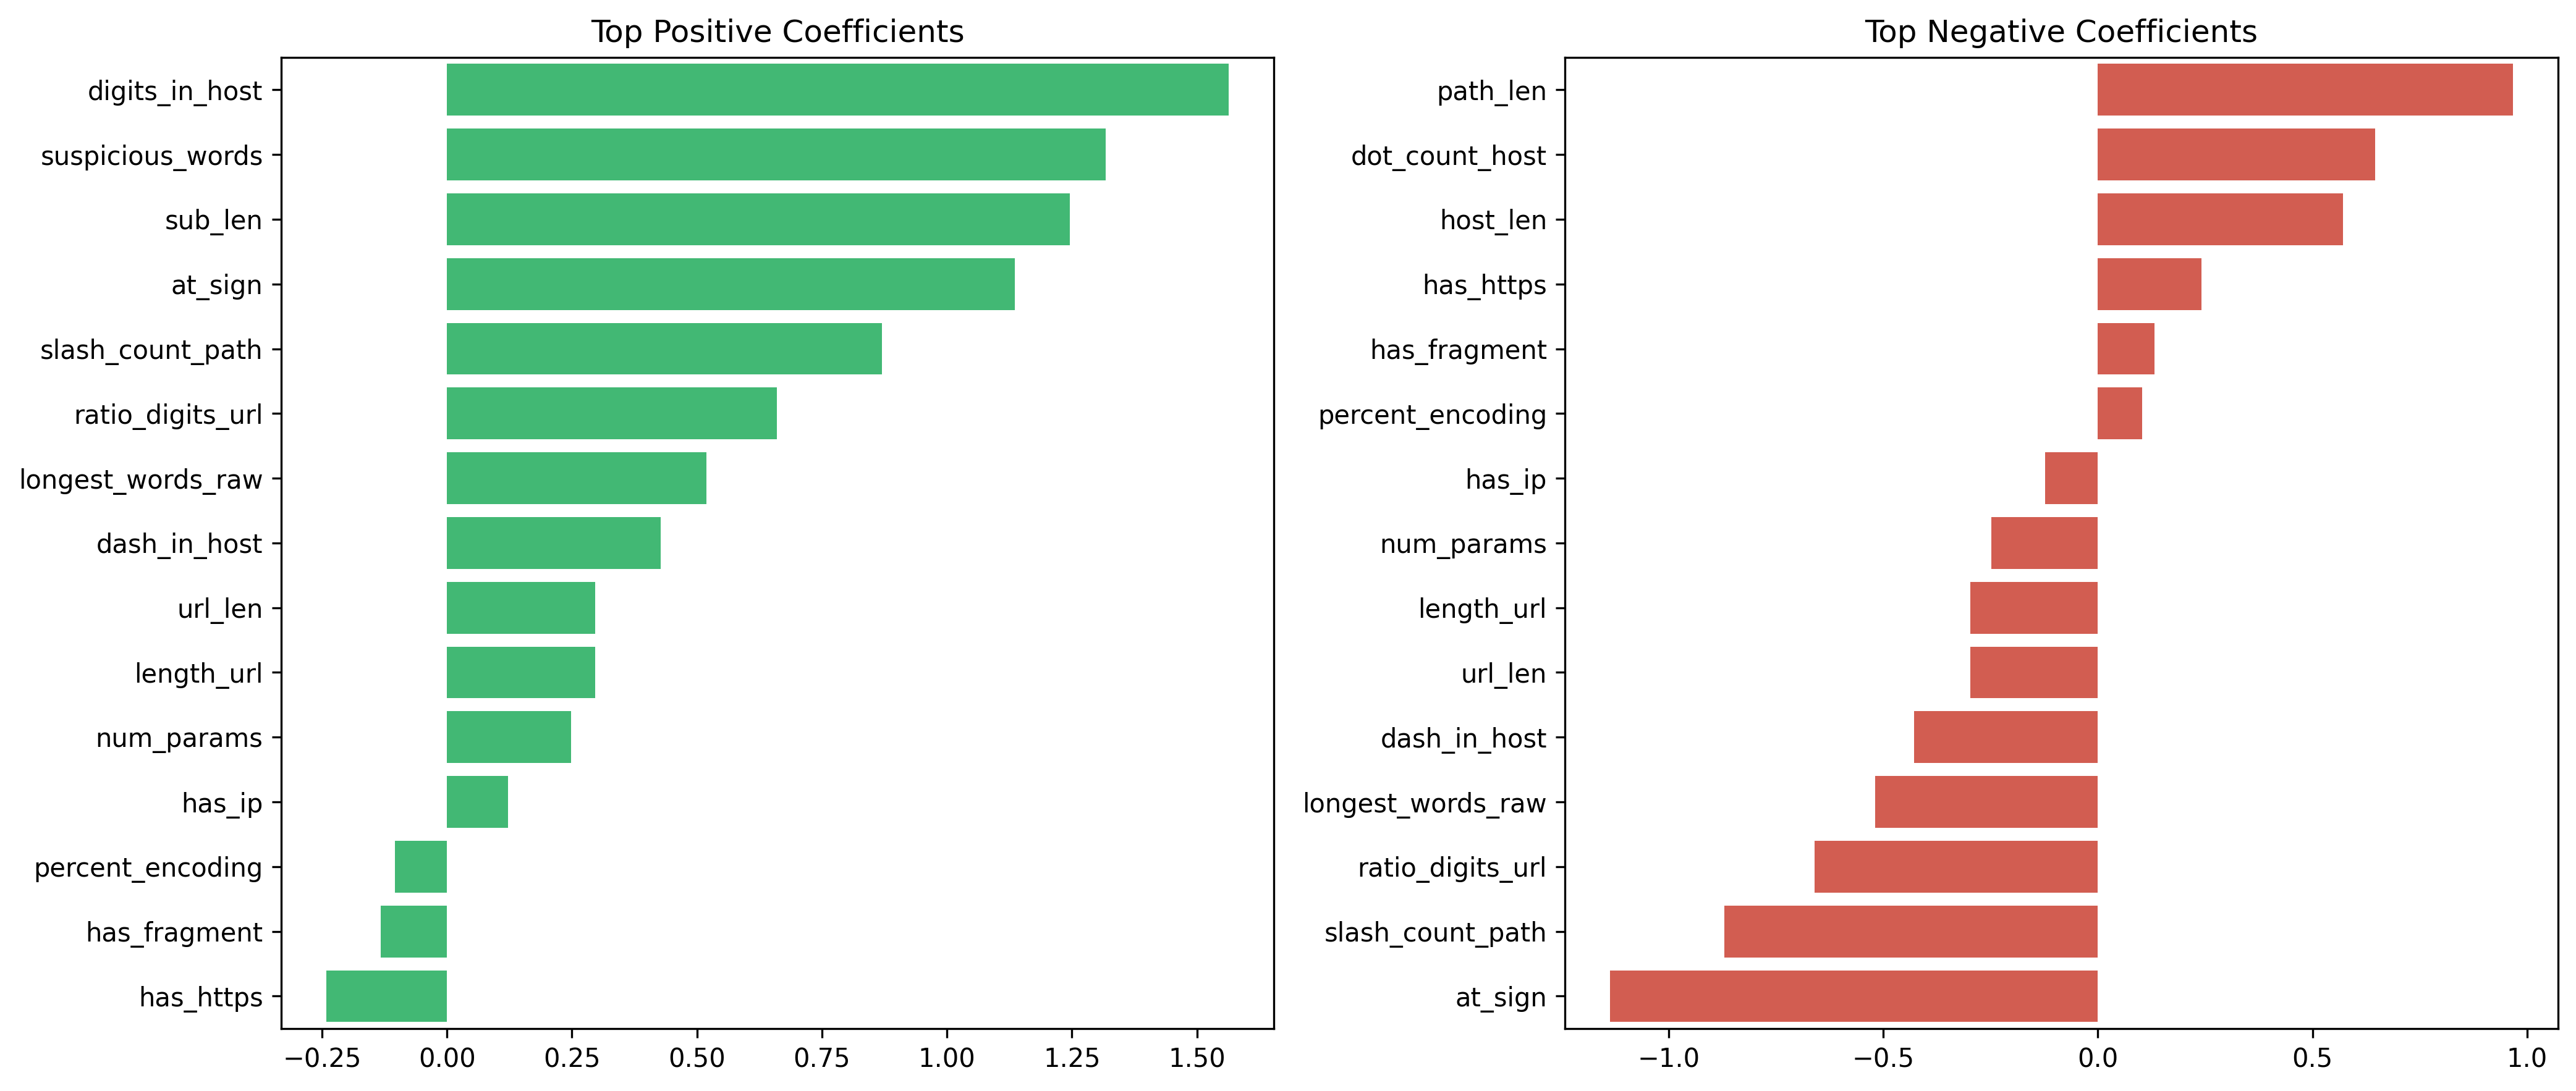
\includegraphics[width=0.48\textwidth]{figures/q2_lr_feature_importance.png}
\caption{Top positive/negative Logistic Regression coefficients.}
\label{fig:q2-coef}
\end{figure}

Figures~\ref{fig:q2-roc} and \ref{fig:q2-pr} indicate stronger ranking consistency for Logistic Regression. The coefficient view in Figure~\ref{fig:q2-coef} also confirms that multiple feature families contribute, validating the combined-feature strategy.

\subsection{Model Tradeoff Interpretation}

Naive Bayes demonstrates a conservative positive prediction tendency in this dataset, reflected by high precision but low recall. Logistic Regression provides a better balance and higher F1-score, which is generally more desirable when both false alarms and misses are costly.

From an operational perspective:
\begin{itemize}
    \item If minimizing false positives is the primary objective, Naive Bayes can be acceptable with threshold tuning.
    \item If balanced detection quality is required, Logistic Regression with combined features is the preferred choice.
\end{itemize}
